%% Title of the paper:
\newcommand{\hemaClassTitle}{\hemaClass{}: Online one-by-one normalization and classification of hematological malignacies}

% Load packages
\usepackage{fullpage} % Larger margins
\usepackage{amssymb,amsmath}
\usepackage{authblk}  % For author affiliations
\usepackage[hypertexnames=false]{hyperref} % For urls and hyperlinks
\usepackage{graphicx}
\usepackage[numbers,sort]{natbib}
\usepackage{cite} % Make references as [1-4], not [1,2,3,4]

% To do notes
\usepackage[
%  disable, %turn off todonotes
  colorinlistoftodos, %enable a coloured square in the list of todos
  textwidth=2cm, %set the width of the todonotes
  textsize=scriptsize, %size of the text in the todonotes
  ]{todonotes}

% Macros
\newcommand{\hemaClass}{\href{http://hemaClass.org}{\texttt{hemaClass.org}}}
\newcommand{\R}{\textsf{R}}
\newcommand{\pkg}[1]{\textbf{#1}}

\DeclareMathOperator*{\median}{median}
\DeclareMathOperator*{\std}{std}

% Hypenation
\hyphenation{Chemo-resistance}


%\begin{document}

\phantomsection
\addcontentsline{toc}{section}{Supplementary Material}
\begin{center}
{\huge SUPPLEMENTARY MATERIAL}\bigskip \\
{\bf \hemaClassTitle{}}
\end{center}

\section{Supplementary figures and tables}
%This section holds the supplementary figures and tables.

\begin{figure*}[htb]
\begin{center}
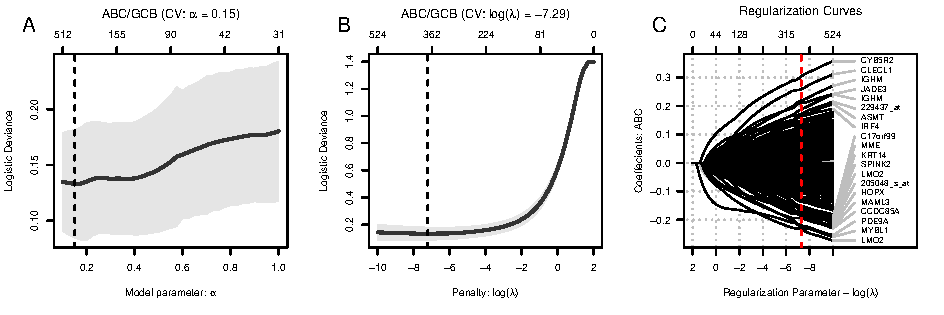
\includegraphics[width=1\textwidth]{figures/figureS1.pdf}
\end{center}
\caption{Ten fold cross validation for the parameters $\alpha$ and $\lambda$ in a logistic regression regularized by elastic net.
In panels A and B the deviance is plotted against the model parameter $\alpha$ and regularization parameter $\lambda$, respectively.
In Panel C the regularization curves are shown.
Black and grey curves represent selected and non-selected probe-sets, respectively.
Positive and negative coefficients indicate that high expression values for the associated gene are related to ABC and GCB, respectively.
The red line indicates the model chosen through $10$ fold cross validation.
The gene symbols for the $20$ probe-sets associated with the largest absolute coefficients in the chosen gene expression predictors are displayed in Panel C.}
\label{fig:crossval}
\end{figure*}

%latex.default(tableS1, file = "tables/tableS1.tex", title = "",     cgroup = names(studies.vec[-5]), rgroup = c("Wright's method",         "One-by-one", "Reference based"), size = "footnotesize",     label = "tab:confusionABCGCBHEMA", caption = caption)%
\begin{table}[!tbp]
{\footnotesize
\caption{Confusion tables for the ABC/GCB classifiers.
The columns represent cohort based normalisation using the ABC/GCB classifier
based on elastic net.
The first part of the table compares Wright's method for ABC/GCB classification
with the elastic net based.
In the second and third part one-by-one and reference based normalisation is
compared to cohort based normalisation using the ABC/GCB classifier based on
elastic net.\label{tab:confusionABCGCBHEMA}} 
\begin{center}
\begin{tabular}{lrrrcrrrcrrrcrrr}
\hline\hline
\multicolumn{1}{l}{\bfseries }&\multicolumn{3}{c}{\bfseries CHEPRETRO}&\multicolumn{1}{c}{\bfseries }&\multicolumn{3}{c}{\bfseries MDFCI}&\multicolumn{1}{c}{\bfseries }&\multicolumn{3}{c}{\bfseries IDRC}&\multicolumn{1}{c}{\bfseries }&\multicolumn{3}{c}{\bfseries LLMPP R-CHOP}\tabularnewline
\cline{2-4} \cline{6-8} \cline{10-12} \cline{14-16}
\multicolumn{1}{l}{}&\multicolumn{1}{c}{ABC}&\multicolumn{1}{c}{NC}&\multicolumn{1}{c}{GCB}&\multicolumn{1}{c}{}&\multicolumn{1}{c}{ABC}&\multicolumn{1}{c}{NC}&\multicolumn{1}{c}{GCB}&\multicolumn{1}{c}{}&\multicolumn{1}{c}{ABC}&\multicolumn{1}{c}{NC}&\multicolumn{1}{c}{GCB}&\multicolumn{1}{c}{}&\multicolumn{1}{c}{ABC}&\multicolumn{1}{c}{NC}&\multicolumn{1}{c}{GCB}\tabularnewline
\hline
{\bfseries Wright's method}&&&&&&&&&&&&&&&\tabularnewline
~~ABC&$38$&$2$&$ 0$&&$28$&$14$&$ 0$&&$174$&$23$&$  1$&&$90$&$ 3$&$  0$\tabularnewline
~~NC&$ 1$&$4$&$ 0$&&$ 1$&$11$&$ 3$&&$  6$&$26$&$ 12$&&$ 6$&$19$&$  8$\tabularnewline
~~GCB&$ 0$&$2$&$42$&&$ 0$&$ 1$&$29$&&$  5$&$31$&$189$&&$ 0$&$ 5$&$102$\tabularnewline
\hline
{\bfseries One-by-one}&&&&&&&&&&&&&&&\tabularnewline
~~ABC&$34$&$0$&$ 0$&&$24$&$ 0$&$ 0$&&$ 95$&$ 0$&$  0$&&$76$&$ 0$&$  0$\tabularnewline
~~NC&$ 5$&$2$&$ 0$&&$ 6$&$ 4$&$ 0$&&$102$&$19$&$  0$&&$20$&$ 6$&$  0$\tabularnewline
~~GCB&$ 0$&$6$&$42$&&$ 0$&$22$&$35$&&$  4$&$67$&$208$&&$ 0$&$21$&$110$\tabularnewline
\hline
{\bfseries Reference based}&&&&&&&&&&&&&&&\tabularnewline
~~ABC&$29$&$6$&$ 0$&&$16$&$ 0$&$ 0$&&$153$&$ 0$&$  0$&&$89$&$22$&$  3$\tabularnewline
~~NC&$ 0$&$1$&$ 4$&&$ 2$&$12$&$ 0$&&$ 32$&$36$&$  0$&&$ 0$&$ 0$&$ 28$\tabularnewline
~~GCB&$ 0$&$0$&$19$&&$ 0$&$ 6$&$25$&&$  0$&$42$&$202$&&$ 0$&$ 0$&$ 61$\tabularnewline
\hline
\end{tabular}\end{center}}

\end{table}

%latex.default(tableS2, file = "tables/tableS2.tex", title = "",     rgroup = flip(studies.vec)[names(subtab)], cgroup = c("One-by-one normalisation",         "Reference based"), size = "small", label = "tab:BAGShemaclass",     caption = caption)%
\begin{table}[!tbp]
{\small
\caption{Confusion tables for the BAGS classifier. One-by-one and reference
based normalisation are shown in the columns and cohort normalisation in the
rows.\label{tab:BAGShemaclass}} 
\begin{center}
\begin{tabular}{lrrrrrrcrrrrrr}
\hline\hline
\multicolumn{1}{l}{\bfseries }&\multicolumn{6}{c}{\bfseries One-by-one normalisation}&\multicolumn{1}{c}{\bfseries }&\multicolumn{6}{c}{\bfseries Reference based}\tabularnewline
\cline{2-7} \cline{9-14}
\multicolumn{1}{l}{}&\multicolumn{1}{c}{N}&\multicolumn{1}{c}{CB}&\multicolumn{1}{c}{CC}&\multicolumn{1}{c}{M}&\multicolumn{1}{c}{PB}&\multicolumn{1}{c}{UC}&\multicolumn{1}{c}{}&\multicolumn{1}{c}{N}&\multicolumn{1}{c}{CB}&\multicolumn{1}{c}{CC}&\multicolumn{1}{c}{M}&\multicolumn{1}{c}{PB}&\multicolumn{1}{c}{UC}\tabularnewline
\hline
{\bfseries CHEPRETRO}&&&&&&&&&&&&&\tabularnewline
~~Naive&$1$&$ 0$&$  0$&$0$&$ 0$&$ 1$&&$ 2$&$ 0$&$  0$&$ 0$&$ 0$&$ 0$\tabularnewline
~~Centroblast&$0$&$18$&$  0$&$0$&$ 0$&$ 0$&&$ 0$&$ 4$&$  4$&$ 0$&$ 0$&$ 1$\tabularnewline
~~Centrocyte&$0$&$10$&$ 11$&$0$&$ 5$&$ 9$&&$ 0$&$ 0$&$ 25$&$ 1$&$ 0$&$ 0$\tabularnewline
~~Memory&$0$&$ 0$&$  0$&$3$&$ 0$&$ 1$&&$ 0$&$ 0$&$  0$&$ 2$&$ 0$&$ 0$\tabularnewline
~~Plasmablast&$0$&$ 0$&$  0$&$0$&$16$&$ 0$&&$ 0$&$ 0$&$  0$&$ 0$&$ 8$&$ 3$\tabularnewline
~~Unclassified&$0$&$ 7$&$  0$&$0$&$ 4$&$ 3$&&$ 0$&$ 0$&$  2$&$ 2$&$ 0$&$ 5$\tabularnewline
\hline
{\bfseries MDFCI}&&&&&&&&&&&&&\tabularnewline
~~Naive&$1$&$ 1$&$  0$&$1$&$ 2$&$ 3$&&$ 3$&$ 0$&$  0$&$ 1$&$ 0$&$ 2$\tabularnewline
~~Centroblast&$0$&$18$&$  0$&$0$&$ 1$&$ 0$&&$ 0$&$ 9$&$  0$&$ 0$&$ 0$&$ 3$\tabularnewline
~~Centrocyte&$0$&$ 7$&$  8$&$2$&$10$&$ 6$&&$ 0$&$ 0$&$ 22$&$ 1$&$ 0$&$ 1$\tabularnewline
~~Memory&$0$&$ 0$&$  0$&$6$&$ 0$&$ 0$&&$ 0$&$ 0$&$  0$&$ 5$&$ 0$&$ 0$\tabularnewline
~~Plasmablast&$0$&$ 0$&$  0$&$0$&$11$&$ 0$&&$ 0$&$ 0$&$  0$&$ 0$&$ 7$&$ 0$\tabularnewline
~~Unclassified&$0$&$ 1$&$  0$&$1$&$ 7$&$ 5$&&$ 1$&$ 0$&$  0$&$ 2$&$ 1$&$ 3$\tabularnewline
\hline
{\bfseries IDRC}&&&&&&&&&&&&&\tabularnewline
~~Naive&$0$&$ 0$&$  3$&$0$&$ 6$&$ 4$&&$12$&$ 0$&$  0$&$ 0$&$ 1$&$ 0$\tabularnewline
~~Centroblast&$0$&$16$&$ 27$&$0$&$27$&$22$&&$ 2$&$62$&$  2$&$ 0$&$ 5$&$12$\tabularnewline
~~Centrocyte&$0$&$ 0$&$140$&$0$&$39$&$18$&&$ 1$&$ 2$&$146$&$ 7$&$ 8$&$18$\tabularnewline
~~Memory&$0$&$ 0$&$  1$&$8$&$20$&$10$&&$ 0$&$ 0$&$  0$&$35$&$ 3$&$ 1$\tabularnewline
~~Plasmablast&$0$&$ 0$&$  1$&$0$&$74$&$ 4$&&$ 0$&$ 0$&$  0$&$ 1$&$76$&$ 1$\tabularnewline
~~Unclassified&$0$&$ 0$&$ 14$&$0$&$44$&$17$&&$ 7$&$ 0$&$  0$&$ 9$&$16$&$38$\tabularnewline
\hline
{\bfseries LLMPP R-CHOP}&&&&&&&&&&&&&\tabularnewline
~~Naive&$1$&$ 2$&$  0$&$0$&$ 5$&$ 6$&&$ 8$&$ 0$&$  0$&$ 1$&$ 0$&$ 1$\tabularnewline
~~Centroblast&$0$&$32$&$  0$&$0$&$ 2$&$ 7$&&$ 0$&$37$&$  1$&$ 0$&$ 0$&$ 1$\tabularnewline
~~Centrocyte&$0$&$ 5$&$ 54$&$0$&$18$&$12$&&$ 0$&$ 1$&$ 66$&$ 1$&$ 1$&$ 4$\tabularnewline
~~Memory&$0$&$ 0$&$  0$&$5$&$13$&$ 4$&&$ 0$&$ 0$&$  0$&$22$&$ 0$&$ 0$\tabularnewline
~~Plasmablast&$0$&$ 0$&$  0$&$0$&$32$&$ 0$&&$ 0$&$ 0$&$  0$&$ 1$&$24$&$ 4$\tabularnewline
~~Unclassified&$0$&$ 2$&$  0$&$0$&$27$&$ 6$&&$ 7$&$ 1$&$  0$&$ 1$&$ 0$&$21$\tabularnewline
\hline
\end{tabular}\end{center}}

\end{table}

%latex.default(tableS3, file = "tables/tableS3.tex", title = "",     rgroup = names(subtab$onebyone), cgroup = flip(studies.vec)[names(subtab$onebyone[[1]])],     size = "small", label = "tab:confusiondrugonebyone", caption = captionS3)%
\begin{table}[!tbp]
\begin{adjustwidth}{-1in}{0in}
{\small
\caption{Confusion tables for the REGS classifiers.
One-by-one normalization are shown in the rows and cohort normalization in the
columns.\label{tab:confusiondrugonebyone}} 
\begin{center}
\begin{tabular}{lrrrcrrrcrrrcrrr}
\hline\hline
\multicolumn{1}{l}{\bfseries }&\multicolumn{3}{c}{\bfseries CHEPRETRO}&\multicolumn{1}{c}{\bfseries }&\multicolumn{3}{c}{\bfseries MDFCI}&\multicolumn{1}{c}{\bfseries }&\multicolumn{3}{c}{\bfseries IDRC}&\multicolumn{1}{c}{\bfseries }&\multicolumn{3}{c}{\bfseries LLMPP R-CHOP}\tabularnewline
\cline{2-4} \cline{6-8} \cline{10-12} \cline{14-16}
\multicolumn{1}{l}{}&\multicolumn{1}{c}{Sen}&\multicolumn{1}{c}{Int}&\multicolumn{1}{c}{Res}&\multicolumn{1}{c}{}&\multicolumn{1}{c}{Sen}&\multicolumn{1}{c}{Int}&\multicolumn{1}{c}{Res}&\multicolumn{1}{c}{}&\multicolumn{1}{c}{Sen}&\multicolumn{1}{c}{Int}&\multicolumn{1}{c}{Res}&\multicolumn{1}{c}{}&\multicolumn{1}{c}{Sen}&\multicolumn{1}{c}{Int}&\multicolumn{1}{c}{Res}\tabularnewline
\hline
{\bfseries Cyclophosphamide}&&&&&&&&&&&&&&&\tabularnewline
~~Sensitive&$40$&$ 1$&$ 0$&&$34$&$ 5$&$ 0$&&$178$&$  0$&$  0$&&$108$&$ 2$&$ 0$\tabularnewline
~~Intermediate&$ 6$&$17$&$ 0$&&$ 0$&$15$&$ 6$&&$114$&$  0$&$  0$&&$  8$&$32$&$ 1$\tabularnewline
~~Resistant&$ 0$&$ 3$&$22$&&$ 0$&$ 1$&$30$&&$203$&$  0$&$  0$&&$  0$&$15$&$67$\tabularnewline
\hline
{\bfseries Doxorubicin}&&&&&&&&&&&&&&&\tabularnewline
~~Sensitive&$30$&$ 0$&$ 0$&&$29$&$ 0$&$ 0$&&$ 25$&$ 86$&$ 39$&&$ 77$&$ 0$&$ 0$\tabularnewline
~~Intermediate&$21$&$ 6$&$ 0$&&$32$&$ 0$&$ 0$&&$  0$&$  6$&$170$&&$ 78$&$ 1$&$ 0$\tabularnewline
~~Resistant&$ 0$&$14$&$18$&&$ 6$&$12$&$12$&&$  0$&$  0$&$169$&&$ 13$&$43$&$21$\tabularnewline
\hline
{\bfseries Vincristine}&&&&&&&&&&&&&&&\tabularnewline
~~Sensitive&$36$&$ 0$&$ 0$&&$33$&$ 0$&$ 0$&&$ 42$&$ 90$&$ 33$&&$ 78$&$ 0$&$ 0$\tabularnewline
~~Intermediate&$ 7$&$ 9$&$ 0$&&$24$&$ 2$&$ 0$&&$  1$&$ 17$&$136$&&$ 59$&$15$&$ 0$\tabularnewline
~~Resistant&$ 1$&$10$&$26$&&$ 1$&$15$&$16$&&$  1$&$  3$&$172$&&$ 11$&$36$&$34$\tabularnewline
\hline
{\bfseries Combined}&&&&&&&&&&&&&&&\tabularnewline
~~Sensitive&$32$&$ 0$&$ 0$&&$33$&$ 0$&$ 0$&&$135$&$ 14$&$  1$&&$ 87$&$ 0$&$ 0$\tabularnewline
~~Intermediate&$19$&$ 9$&$ 0$&&$27$&$ 1$&$ 0$&&$ 19$&$143$&$ 21$&&$ 70$&$ 0$&$ 0$\tabularnewline
~~Resistant&$ 0$&$13$&$16$&&$ 3$&$13$&$14$&&$  0$&$ 27$&$135$&&$ 16$&$42$&$18$\tabularnewline
\hline
\end{tabular}\end{center}}
\end{adjustwidth}
\end{table}

%latex.default(tableS4, file = "tables/tableS4.tex", title = "",     rgroup = names(subtab$refbased), cgroup = flip(studies.vec)[names(subtab$refbased[[1]])],     size = "small", label = "tab:confusiondrugreference", caption = captionS4)%
\begin{table}[!tbp]
{\small
\caption{Confusion tables for the REGS classifiers.
Reference based normalisation are shown in the rows and cohort normalisation in
the columns. Note, 30 samples were used as reference data and hence not present
in this table.\label{tab:confusiondrugreference}} 
\begin{center}
\begin{tabular}{lrrrcrrrcrrrcrrr}
\hline\hline
\multicolumn{1}{l}{\bfseries }&\multicolumn{3}{c}{\bfseries CHEPRETRO}&\multicolumn{1}{c}{\bfseries }&\multicolumn{3}{c}{\bfseries MDFCI}&\multicolumn{1}{c}{\bfseries }&\multicolumn{3}{c}{\bfseries IDRC}&\multicolumn{1}{c}{\bfseries }&\multicolumn{3}{c}{\bfseries LLMPP R-CHOP}\tabularnewline
\cline{2-4} \cline{6-8} \cline{10-12} \cline{14-16}
\multicolumn{1}{l}{}&\multicolumn{1}{c}{Sen}&\multicolumn{1}{c}{Int}&\multicolumn{1}{c}{Res}&\multicolumn{1}{c}{}&\multicolumn{1}{c}{Sen}&\multicolumn{1}{c}{Int}&\multicolumn{1}{c}{Res}&\multicolumn{1}{c}{}&\multicolumn{1}{c}{Sen}&\multicolumn{1}{c}{Int}&\multicolumn{1}{c}{Res}&\multicolumn{1}{c}{}&\multicolumn{1}{c}{Sen}&\multicolumn{1}{c}{Int}&\multicolumn{1}{c}{Res}\tabularnewline
\hline
{\bfseries Cyclophosphamide}&&&&&&&&&&&&&&&\tabularnewline
~~Sensitive&$13$&$10$&$ 0$&&$26$&$ 4$&$ 0$&&$134$&$ 32$&$  0$&&$89$&$ 5$&$ 0$\tabularnewline
~~Intermediate&$ 0$&$ 7$&$10$&&$ 0$&$10$&$ 1$&&$  3$&$ 77$&$ 29$&&$ 0$&$27$&$ 9$\tabularnewline
~~Resistant&$ 0$&$ 0$&$19$&&$ 0$&$ 0$&$20$&&$  0$&$  9$&$181$&&$ 0$&$ 2$&$71$\tabularnewline
\hline
{\bfseries Doxorubicin}&&&&&&&&&&&&&&&\tabularnewline
~~Sensitive&$18$&$ 2$&$ 0$&&$19$&$ 0$&$ 0$&&$132$&$  7$&$  0$&&$50$&$15$&$ 0$\tabularnewline
~~Intermediate&$ 0$&$14$&$ 2$&&$ 0$&$21$&$ 0$&&$ 24$&$143$&$  3$&&$ 0$&$55$&$13$\tabularnewline
~~Resistant&$ 0$&$ 0$&$23$&&$ 0$&$ 3$&$18$&&$  0$&$ 16$&$140$&&$ 0$&$ 0$&$70$\tabularnewline
\hline
{\bfseries Vincristine}&&&&&&&&&&&&&&&\tabularnewline
~~Sensitive&$18$&$ 5$&$ 0$&&$16$&$ 6$&$ 0$&&$127$&$ 32$&$  0$&&$71$&$ 0$&$ 0$\tabularnewline
~~Intermediate&$ 0$&$10$&$ 1$&&$ 0$&$ 8$&$ 9$&&$ 12$&$ 83$&$ 46$&&$ 9$&$49$&$ 0$\tabularnewline
~~Resistant&$ 0$&$ 0$&$25$&&$ 0$&$ 0$&$22$&&$  1$&$ 10$&$154$&&$ 0$&$10$&$64$\tabularnewline
\hline
{\bfseries Combined}&&&&&&&&&&&&&&&\tabularnewline
~~Sensitive&$19$&$ 3$&$ 0$&&$23$&$ 1$&$ 0$&&$125$&$ 14$&$  0$&&$64$&$12$&$ 0$\tabularnewline
~~Intermediate&$ 0$&$11$&$ 5$&&$ 0$&$16$&$ 0$&&$ 12$&$148$&$ 14$&&$ 0$&$46$&$10$\tabularnewline
~~Resistant&$ 0$&$ 0$&$21$&&$ 0$&$ 0$&$21$&&$  0$&$  6$&$146$&&$ 0$&$ 0$&$71$\tabularnewline
\hline
\end{tabular}\end{center}}

\end{table}

% latex table generated in R 3.3.1 by xtable 1.8-2 package
% Fri Aug 19 11:39:25 2016
\begin{table}[ht]
\centering
\begin{tabular}{lrrr}
  \hline
Classifier & nProbes & nHGNC & nEnsembl \\ 
  \hline
ABC/GCB & 381 & 291 & 273 \\ 
  BAGS & 327 & 224 & 205 \\ 
  Vincristine Classifier & 33 & 32 & 29 \\ 
  Vincristine Predictor & 22 & 21 & 18 \\ 
  Cyclophosphamide Classifier & 74 & 73 & 66 \\ 
  Cyclophosphamide Predictor & 28 & 27 & 25 \\ 
  Doxorubicine Classifier & 119 & 118 & 112 \\ 
  Doxorubicine Predictor & 53 & 52 & 48 \\ 
  Combined Classifier & 203 & 202 & 185 \\ 
  Combined Predictor & 90 & 88 & 80 \\ 
   \hline
\end{tabular}
\caption{Number of probes used in the classifiers and the number of corresponding HGNC and Ensembl gene IDs} 
\label{probeTable}
\end{table}


\clearpage



\section{Graham's formula}
\label{sec:graham}
This section derives Graham's formula which, in our context, yields the posterior probability of resistance to the combination of multiple drugs, given resistance to the individual drugs.
For simplicity, the formula is derived for two drugs.
The formula straightforwardly generalizes to three or more drugs.

Let $C$, $H$, and $B$ be Bernoulli distributed random variables with probability parameter $1/2$, where
$C = 1$ indicates resistance to Cyclophosphamide $C$,
$H = 1$ indicates resistance to Doxorubicin $H$, and
$B = 1$ indicates resistance to the combination of $H$ and $C$.
Conversely, $C,H,$ and $B = 0$ indicate sensitivity towards $C,H,$ and $B$, respectively.
Under an assumption of conditional drug independence
\begin{align*}
  P(C=1, H=1| B=1) &= P(C=1 | B=1) P(H=1 | B=1), \text{ and } \\
  P(C=1, H=1| B=0) &= P(C=1 | B=0) P(H=1 | B=0)
\end{align*}
we have that
\begin{align*}
  &P(B=1 | H=1, C=1)
  \\&\qquad
   = \frac{P(C=1, H=1, B=1)}
          {P(C=1, H=1)}
  \\&\qquad
   = \frac{P(C=1, H=1 | B=1) P(B=1)}
          {P(C=1, H=1, B=1) + P(C=1, H=1, B=0)}
  \\&\qquad
   = \frac{P(C=1 | B=1) P(H=1 | B=1) P(B=1)}
          {P(C=1, H=1 | B=1) P(B=1) + P(H=1, C=1| B=0) P(B=0)},
\end{align*}
by the definition of conditional probabilities, the law of total probability, and the assumptions.
From the distributional assumption on $B$, $P(B=0) = P(B=1) = 1/2$, and the above then simplifies to:
\begin{equation*}
  P(B=1 | H=1, C=1)
   = \frac{P(C=1 | B=1) P(H=1 | B=1)}
          {P(C=1, H=1 | B=1) + P(H=1, C=1 | B=0)}.
\end{equation*}
For notational convenience, we abbreviate
$P_C = P(C=1 | B=1)$,
$P_H = P(H=1 | B=1)$,
$P_{CH} = P(B=1 | H=1, C=1)$.
The distributional assumptions then imply:
\begin{align*}
  P_{CH}
  &= \frac{P_C P_H}
          {P_C P_H + P(C=1 | B=0) P(H=1 | B=0)}
  \\
  &= \frac{P_C P_H}
          {P_C P_H + P(B=0 | C=1) P(B=0 | H=1)}
  \\
  &= \frac{P_C P_H}
          {P_C P_H + \bigl(1 - P(B=1 | C=1)\bigr)\bigl(1 - P(B=1 | H=1)\bigr)}
  \\
  &= \frac{P_C P_H}
          {P_C P_H + (1 - P_C)(1 - P_H)},
\end{align*}
which is the two-drug equivalent to the used formula.




\section{RMA normalization} \label{supprma}
Recall that ordinary robust multichip average (RMA) pre-processing consists of three steps: (1) Background adjustment, (2) quantile normalization, and (3) summarization of probes to probe-sets, see e.g.\ \citep{Irizarry2003, Irizarry2003b}. For completeness we review ordinary cohort based RMA normalization.

\subsection{Background correction}
In order to produce background adjusted probe intensities we will use the within array normal-exponential de-convolution scheme as implemented by the \texttt{rma.background.correct} command in the Bioconductor package \texttt{preprocessCores}, see
\citep{Irizarry2003b,Bolstad2004}.


\subsection{Quantile normalization}
Let $x_{ijk}$ be the $\log_2$-transformed and background adjusted cohort data, where $i = 1,\dots,I$ index the arrays of the cohort data, $j=1,\dots,J$  index the probe-sets, and $k=1,\dots,K_j$ index the probes nested within probe-sets.

Furthermore, let $G_i$ denote the empirical cumulative distribution function (ECDF) of the probes $\{x_{ijk}\}_{jk}$ on the $i$'th cohort array and $F$ the ECDF of the across array averaged sample quantiles $\{\bar{x}_{\cdot (jk)}\}_{ij}$, where $\{x_{i(jk)}\}_{jk}$ is the order statistic of all probes on the $i$'th cohort array based on the lexicographic ordering of the indices $\{jk\}$. Then each data point is quantile normalized in the following way
\begin{equation*}
     \tilde{x}_{ijk} = F^{-1}(G_i(x_{ijk})),
\end{equation*}
where $F^{-1}$ is calculated as the quantiles of type 2 \citep{Hyndman1996}.
This step is performed by the \texttt{RMA\_norm} function with option \texttt{generateQuan} equal to one in the \pkg{hemaClass} package.

\subsection{Summarization}

For each probe-set $j$ we let $\mu_{ij}$ represent the $\log_2$-scale expression level for array $i$ and probeset $j$, $\alpha_{jk}$ the probe affinity effect, and the $\epsilon_{ijk}$'s are independent identically distributed  error terms with mean 0 and formulate the following linear additive model
\begin{equation*}
   \tilde{x}_{ijk} = \mu_{ij} + \alpha_{jk}+ \epsilon_{ijk},
\end{equation*}
where $\sum_{k=0}^{n_j} \alpha_{jk} = 0$ for all probe-sets. The parameters are estimated by median polish \citep{Holder2001}. The probe affinity estimates are denoted by $\hat{\alpha}_{jk}$.

The RMA normalized cohort data are then given by
\begin{equation*}
   \hat{x}_{ij} = \hat{\mu}_{ij}.
\end{equation*}
This step is performed by the \texttt{RMA\_sum} function in the \hemaClass{} package.




\section{One-by-one RMA normalization of user supplied data}
\subsection{Background correction}

The background correction in one-by-one RMA normalization is unaltered as it is already works in a one-by-one fashion.


\subsection{Quantile normalization}

Let $x_{ijk}$ be the $\log_2$-transformed and background corrected reference data, where $i = 1,\dots,I_R$ index the arrays of the reference data, $j=1,\dots,J$ index the probe-sets, and $k=1,\dots,K_j$ index the probes.
Assume $x_{ijk}$ has been RMA normalized as described above.
Similarly, let $y_{ijk}$ be the log2-transformed and background corrected user supplied data, where $i = 1,\dots,I_U$ index the arrays of the user supplied data, $j=1,\dots,J$  index the probe-sets, and $k=1,\dots,K_j$ index the probes.
Furthermore, let $H_i$ denote the ECDF of the user supplied data $\{y_{ijk}\}_{jk}$.

As quantile normalizer the ECDF of the background corrected reference data is used in place of the ususally applied ECDF of the mean of the sample quantiles
\begin{equation*}
   \tilde{y}_{ijk} = F^{-1}(H_i(y_{ijk})).
\end{equation*}
This step is performed by the \texttt{RMA\_norm} function with options \texttt{generateQuan} equal to zero and \texttt{quantile} equal to the quantiles of the reference data in the \pkg{hemaClass} package.


\subsection{Summarization}

To mimic the RMA summarization the probe effects estimated by median polish on the reference data is subtracted all probes of the user data
\begin{equation*}
   \hat{y}_{ijk} = \tilde{y}_{ijk} - \hat{\alpha}_{jk}.
\end{equation*}
The pre-processed expression value for each probe-set is then estimated as the median of the associated probes.
\begin{equation*}
   \hat{y}_{ij} = \median_{k \in \{1,\dots,n_j \}} \{ \hat{y}_{ijk} \}.
\end{equation*}


\section{Classification}
To ensure identical classification probabilities whether data is supplied as a cohort or one-by-one, we finally subtract the median of each probe-set in the reference from the corresponding probe-set and scale by the standard deviation of each probe-set in the reference data
\begin{equation*}
  (\hat{y}_{ij} - \hat{x}_{\cdot j})/s_{\cdot j},
\end{equation*}
where
$\hat{x}_{\cdot j} = \median_{i \in \{1,\dots,I_R \}} \{\hat{x}_{ij}\}$ and
$s_{\cdot j} = \sd_{i \in \{1,\dots,I_R\}} \{\hat{x}_{ij}\}$.


\section{Model control of one-by-one RMA normalization} \label{sec_rle}
Given the large difference in misclassifications  between InLab and ExLab one-by-one normalized samples, we would like to be able to distinguish between the two in a setting where we are unsure how closely the RMA reference resembles the samples.

\subsection{Relative Log Expression} 
The relative log expression (RLE)	is a quality measure for microarrays introduced by \mbox{\citet{Bolstad2004b}}. Using the notation from above we define the RLE for probe $j$ on array $i$ following RMA normalization as:
\[
	\textrm{RLE}(\hat{y}_{ij}) = \hat{y}_{ij} - \hat{x}_{\cdot j}
\]
i.e. the difference between the estimated expression for probe $j$ on array $i$ and the median expression for probe $j$ in the cohort. A non-zero median RLE across probes for an array thus indicates differences in the number of up- and downregulated genes, while a large interquartile range (IQR) indicates that most genes on a given array are differentially expressed \mbox{\citep{McCall2011}}. Extreme values of these measures may be used to identify arrays with low-quality data. We propose that they may also be used to evaluate how well a sample resembles a given RMA reference following one-by-one normalization (how well it has been normalized), by substituting the cohort median with the RMA reference median.

\subsection{RLE for separation of InLab and ExLab RMA references} \label{rle_sepa}
For each of the five datasets used in the current study a random subset of 30 samples were extracted and set as an InLab reference. The remaining samples for each dataset where then RMA normalized as a cohort, or one-by-one against the randomly selected InLab reference or against the four other datasets (ExLab). RLE values were calculated in all six scenarios and summarized as the absolute value of the median and IQR for each sample. These values are shown in panel A and B in Figure \ref{fig:chep_rle} to Figure \ref{fig:mdfci_rle}. We find that the RLE values in the InLab one-by-one scenarios more closely resemble the values calculated from cohort normalization than the values from ExLab one-by-one normalization. Furthermore differences between InLab and ExLab RLE values are more pronounced for the IQR of RLE than for the median. ROC curves showing the ability of the RLE median or IQR to distinguish between an InLab or ExLab reference were calculated and plotted using the pROC package version 1.8 \citep{Robin2011} in \R, as shown in panels C and D in Figure \ref{fig:chep_rle} to Figure \ref{fig:mdfci_rle}. The area under the curve (AUC) for the ROC curves confirm the superiority of the RLE IQR for distinguishing between a "correct" reference and a "wrong" reference, i.e. in most cases we observe a higher AUC when using the IQR instead of the median RLE.\\\\
Using Youden's index, which maximizes the sum of sensitivity and specificity, we calculated the optimal threshold for each ROC curve based on the RLE IQR as shown in Table \ref{rleTable}. Calculating the median RLE IQR across all datasets and one-by-one RMA references gives a value of 0.62. By rounding of we set a conservative threshold of 0.6 for reference normalized samples, i.e. if the RLE IQR exceeds this value the array is expected to have been normalized incorrectly.

\begin{figure}[!h]
	\begin{center}
		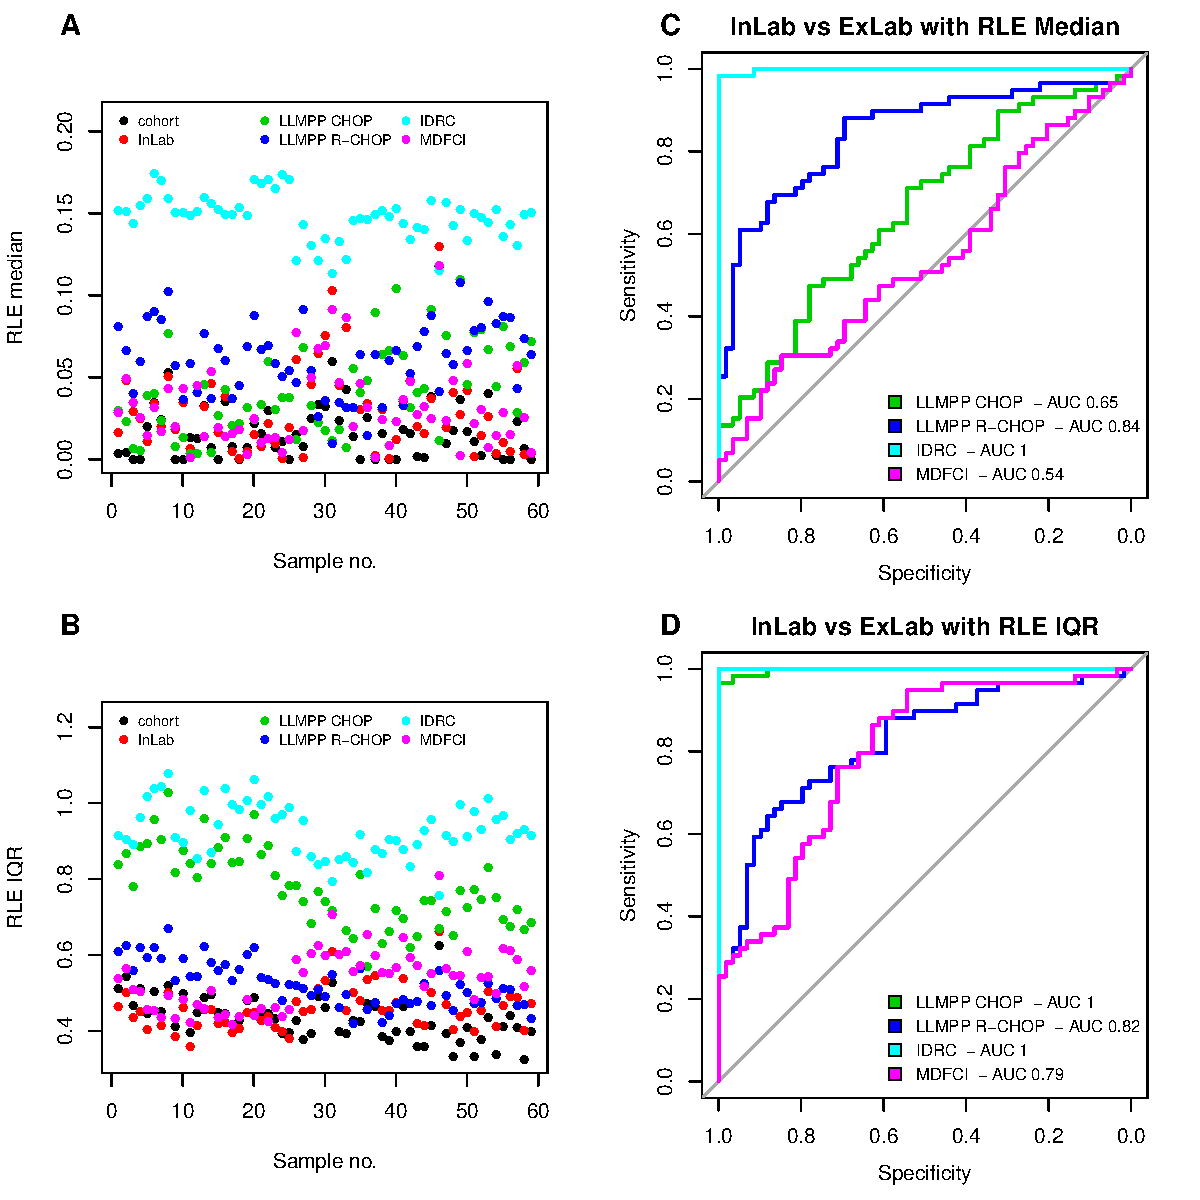
\includegraphics[width=0.8\textwidth]{figures/chep_rle.pdf}
	\end{center}
	\caption{Absolute value of the median (A) and IQR (B) RLE values for different RMA normalizations of the CHEPRETRO dataset and ROC curves for using these values to separate between an InLab and Exlab RMA reference (C,D)}
	\label{fig:chep_rle}
\end{figure}

\begin{figure}[!h]
	\begin{center}
		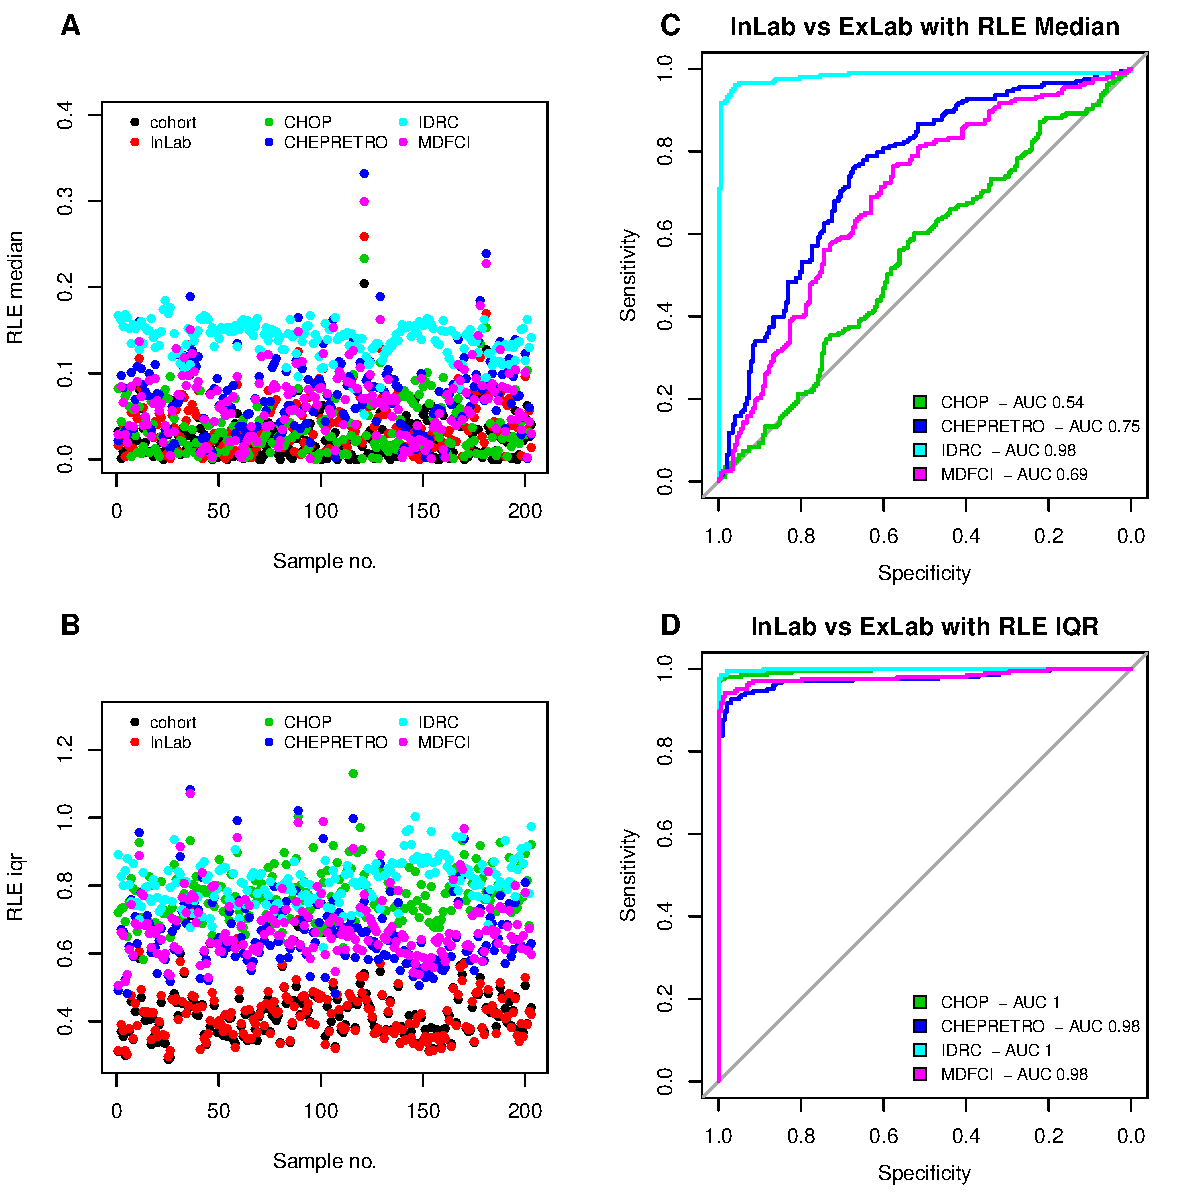
\includegraphics[width=0.8\textwidth]{figures/RCHOP_rle.pdf}
	\end{center}
	\caption{Absolute value of the median (A) and IQR (B) RLE values for different RMA normalizations of the RCHOP dataset and ROC curves for using these values to separate between an InLab and Exlab RMA reference (C,D)}
	\label{fig:rchop_rle}
\end{figure}

\begin{figure}[!h]
	\begin{center}
		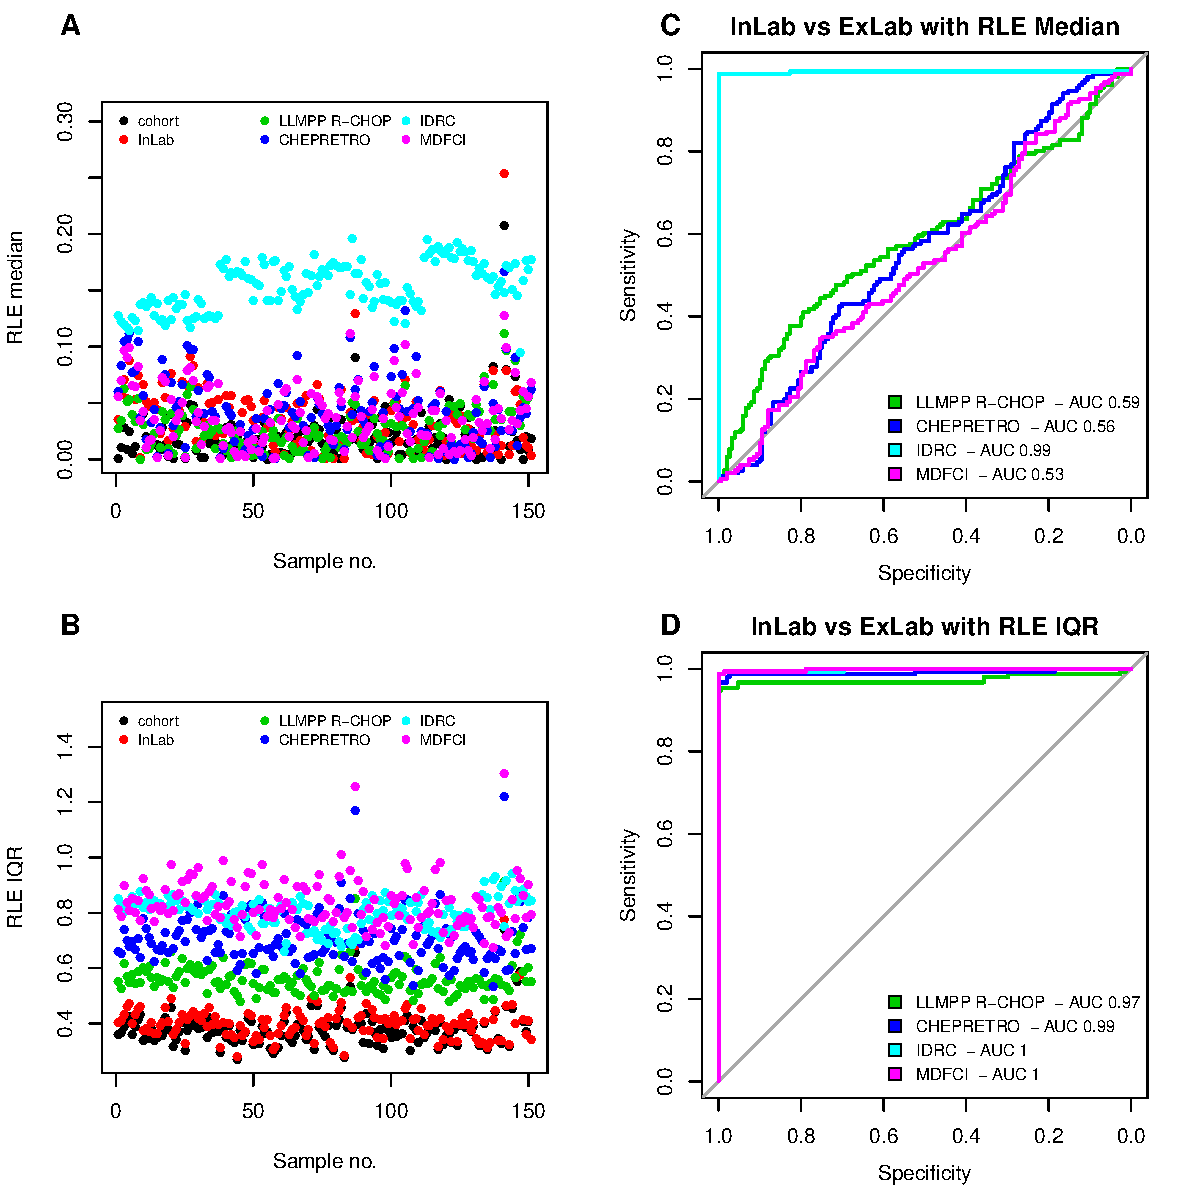
\includegraphics[width=0.8\textwidth]{figures/CHOP_rle.pdf}
	\end{center}
	\caption{Absolute value of the median (A) and IQR (B) RLE values for different RMA normalizations of the CHOP dataset and ROC curves for using these values to separate between an InLab and Exlab RMA reference (C,D)}
	\label{fig:chop_rle}
\end{figure}

\begin{figure}[!h]
	\begin{center}
		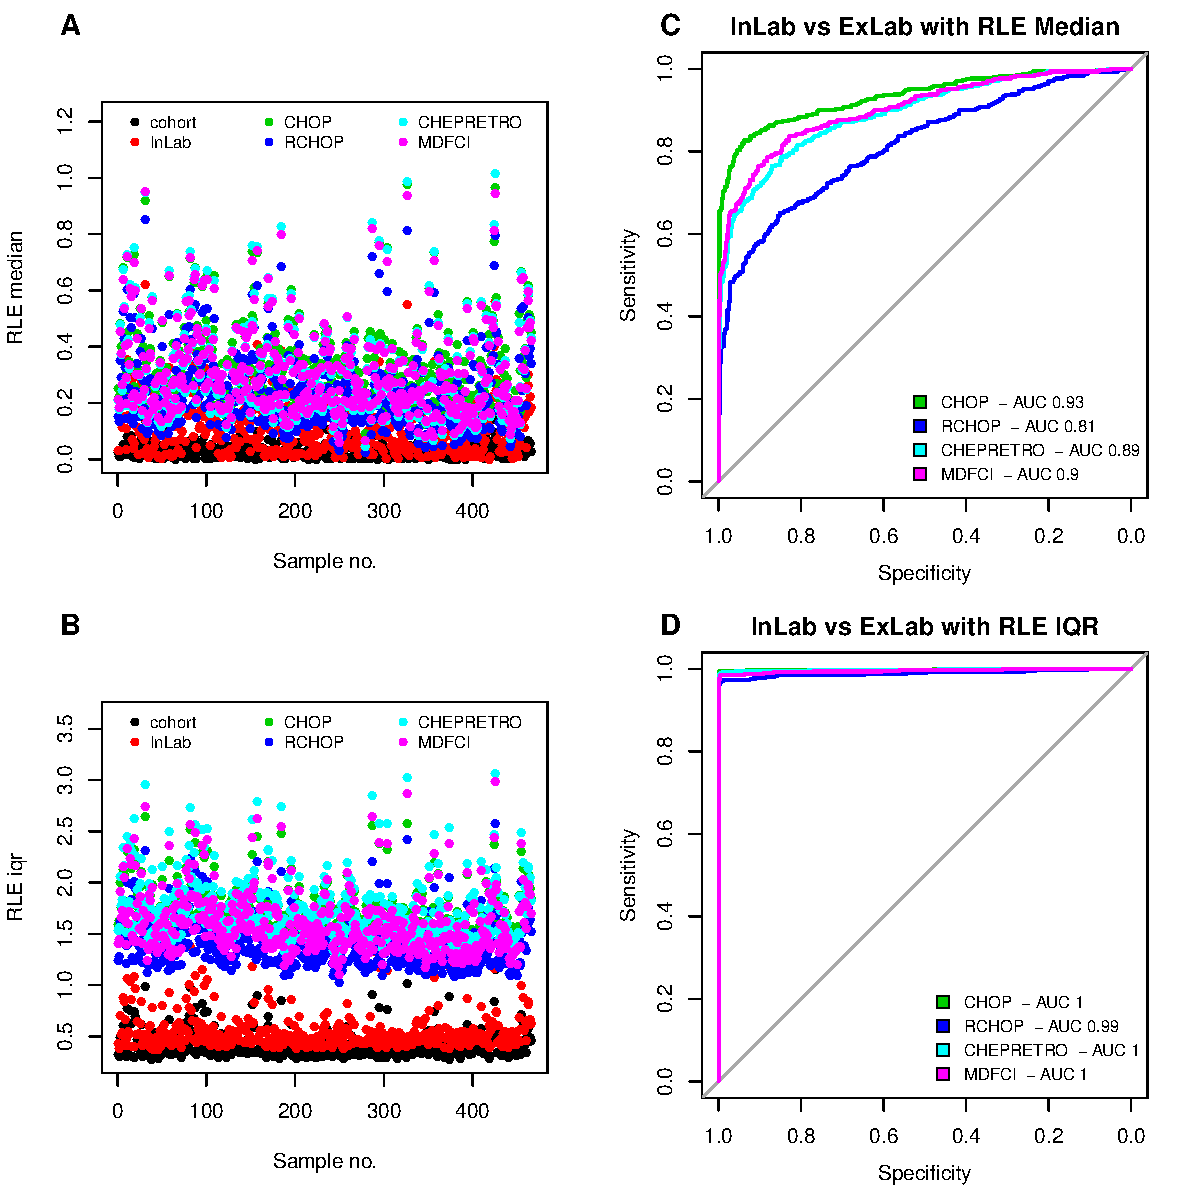
\includegraphics[width=0.8\textwidth]{figures/IDRC_rle.pdf}
	\end{center}
	\caption{Absolute value of the median (A) and IQR (B) RLE values for different RMA normalizations of the IDRC dataset and ROC curves for using these values to separate between an InLab and Exlab RMA reference (C,D)}
	\label{fig:idrc_rle}
\end{figure}

\begin{figure}[!h]
	\begin{center}
		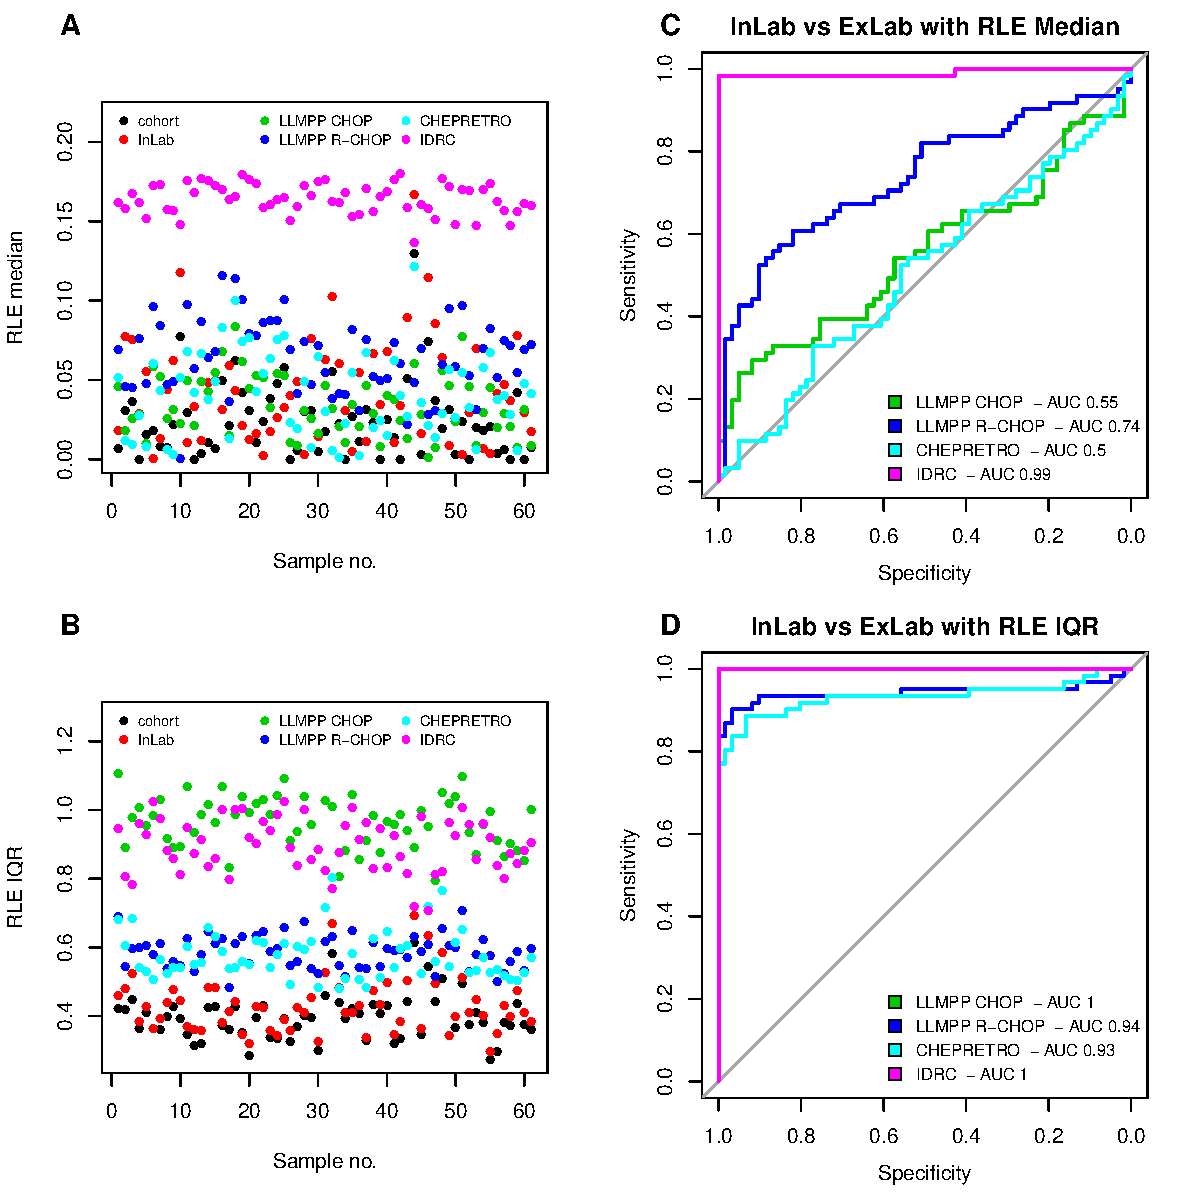
\includegraphics[width=0.8\textwidth]{figures/MDFCI_rle.pdf}
	\end{center}
	\caption{Absolute value of the median (A) and IQR (B) RLE values for different RMA normalizations of the MDFCI dataset and ROC curves for using these values to separate between an InLab and Exlab RMA reference (C,D)}
	\label{fig:mdfci_rle}
\end{figure}

% latex table generated in R 3.3.1 by xtable 1.8-2 package
% Mon Aug 29 13:49:06 2016
\begin{table}[ht]
\centering
\begin{tabular}{llrrr}
  \hline
Dataset & RMA reference & Threshold & Sensitivity & Specificity \\ 
  \hline
CHEPRETRO & LLMPP CHOP & 0.56 & 0.97 & 1.00 \\ 
  CHEPRETRO & LLMPP R-CHOP & 0.47 & 0.68 & 0.85 \\ 
  CHEPRETRO & IDRC & 0.71 & 1.00 & 1.00 \\ 
  CHEPRETRO & MDFCI & 0.54 & 0.95 & 0.54 \\ 
  LLMPP R-CHOP & LLMPP CHOP & 0.61 & 0.98 & 1.00 \\ 
  LLMPP R-CHOP & CHEPRETRO & 0.52 & 0.93 & 0.97 \\ 
  LLMPP R-CHOP & IDRC & 0.68 & 0.99 & 1.00 \\ 
  LLMPP R-CHOP & MDFCI & 0.53 & 0.94 & 0.99 \\ 
  LLMPP CHOP & LLMPP R-CHOP & 0.48 & 0.95 & 0.99 \\ 
  LLMPP CHOP & CHEPRETRO & 0.51 & 0.97 & 1.00 \\ 
  LLMPP CHOP & IDRC & 0.62 & 0.99 & 1.00 \\ 
  LLMPP CHOP & MDFCI & 0.62 & 0.99 & 1.00 \\ 
  IDRC & LLMPP CHOP & 1.39 & 0.99 & 1.00 \\ 
  IDRC & LLMPP R-CHOP & 1.08 & 0.97 & 1.00 \\ 
  IDRC & CHEPRETRO & 1.32 & 0.99 & 1.00 \\ 
  IDRC & MDFCI & 1.19 & 0.98 & 1.00 \\ 
  MDFCI & LLMPP CHOP & 0.74 & 1.00 & 1.00 \\ 
  MDFCI & LLMPP R-CHOP & 0.51 & 0.90 & 0.97 \\ 
  MDFCI & CHEPRETRO & 0.50 & 0.89 & 0.93 \\ 
  MDFCI & IDRC & 0.70 & 1.00 & 1.00 \\ 
  Median & - & 0.62 & 0.97 & 1.00 \\ 
   \hline
\end{tabular}
\caption{Optimal thresholds for RLE IQR} 
\label{rleTable}
\end{table}


\subsection{RLE IQR vs Classification accuracy}
The results in Supplementary Section \ref{rle_sepa} showed that the RLE IQR can be used to determine if samples have been normalized against an Inlab or ExLab reference. In this section we compare the RLE IQR to the classification accuracy. The CHEPRETRO dataset was one-by-one normalized against an InLab reference, the LLMPP CHOP reference, and the LLMPP RCHOP reference, and the LLMPP RCHOP dataset was one-by-one normalized against an InLab reference, the LLMPP CHOP reference, and the CHEPRETREO reference. RLE IQR values were calculated and the proportion of samples below a given threshold and the accuracy (proportion of samples with similar classification in cohort normalized data) were calculated for increasing values of the RLE IQR. This was done for ABC/GCB, BAGS and REGS (CHO) classification. Results are shown in Figure \ref{fig:chep_rle_clas_bags} to Figure \ref{fig:RCHOP_rle_clas_regs}. 

For CHEPRETRO we saw that most samples were retained at the suggested RLE IQR value of 0.6 when samples were normalized against the InLab reference, and a tendency towards higher classification accuracy for samples with low RLE IQR. When normalizing CHEPRETRO against RCHOP the RLE IQR value of 0.6 only excludes a small proportion of the samples and a low accuracy is observed for BAGS and REGS classification while higher accuracies are seen for ABC/GCB. For CHOP normalization most samples are removed at the suggested value, and a high accuracy for the few remaining samples are seen for BAGS and ABC/GCB classification while an accuracy of zero is seen for REGS. 

For the RCHOP dataset most InLab reference normalized samples were retained at the suggested value of 0.6, but lower RLE IQR values did not give higher classification accuracies. Most samples normalized against the CHEPRETRO or CHOP reference are excluded at an RLE IQR of 0.6, but there is no clear indication of higher accuracies for samples with RLE IQR below the threshold.

Looking at results as a whole, a low RLE IQR in itself does not guarantee a higher classification accuracy, but it does exclude most ExLab normalized samples, and accordingly in most cases should exclude samples with low classification accuracy from biased RMA normalization.

\begin{figure}
	\begin{center}
		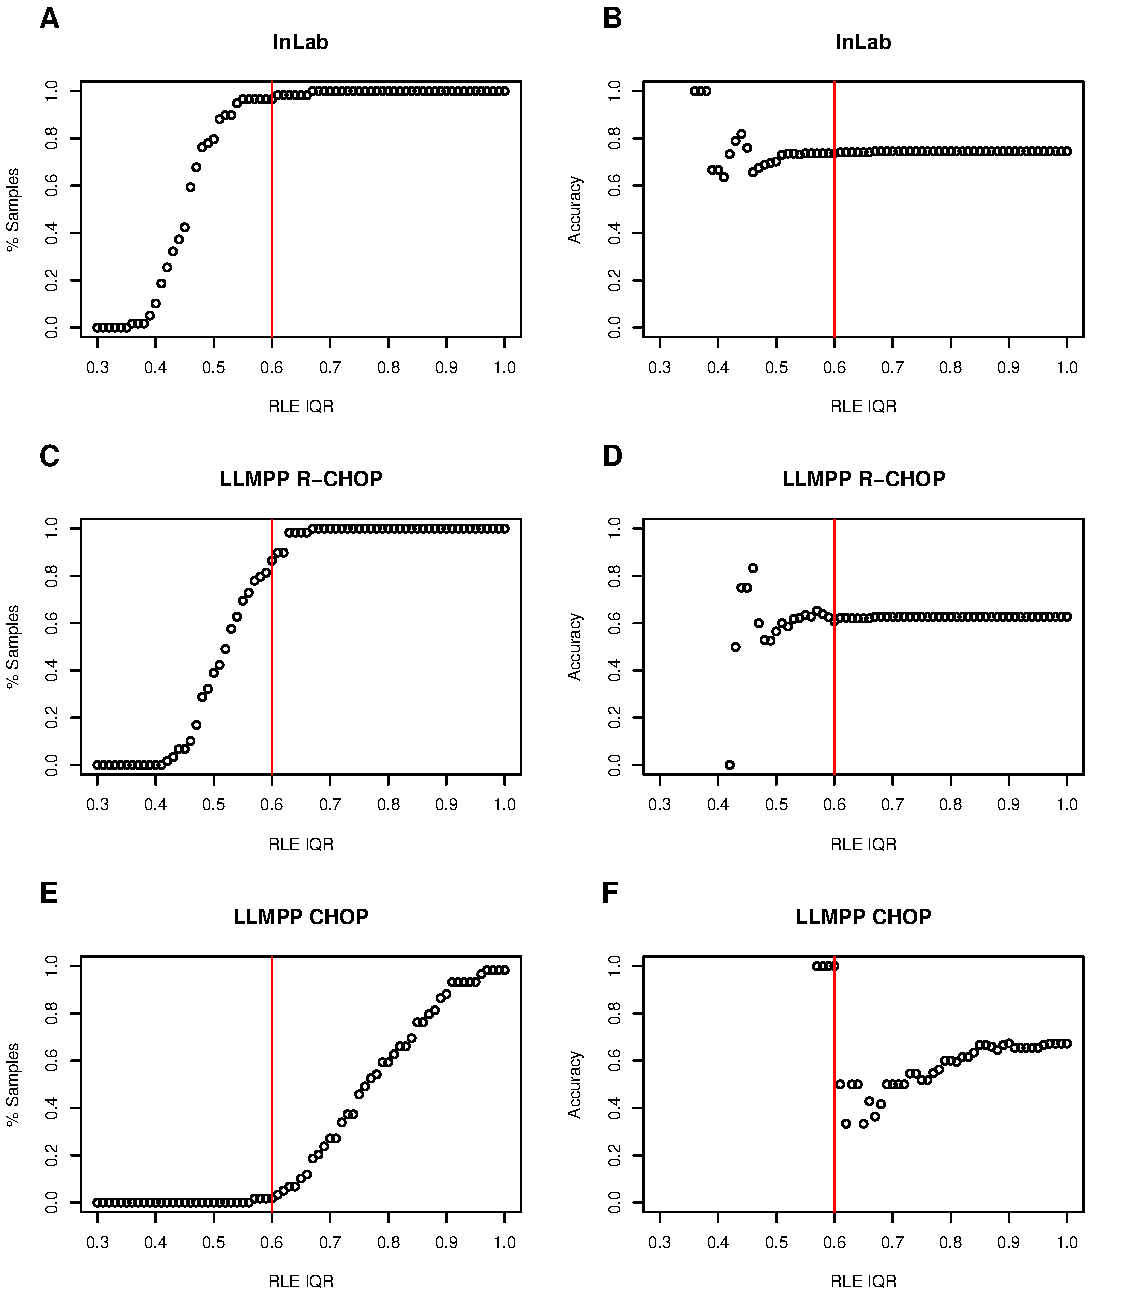
\includegraphics[width=0.8\textwidth]{figures/chep_rle_classification_bags.pdf}
	\end{center}
	\caption{Proportion samples retained and accuracy of BAGS classification (percent similar with cohort based) against increasing RLE IQR thresholds for different references in CHEPRETRO. The vertical line marks the suggested threshold of 0.6}
	\label{fig:chep_rle_clas_bags}
\end{figure}

\begin{figure}
	\begin{center}
		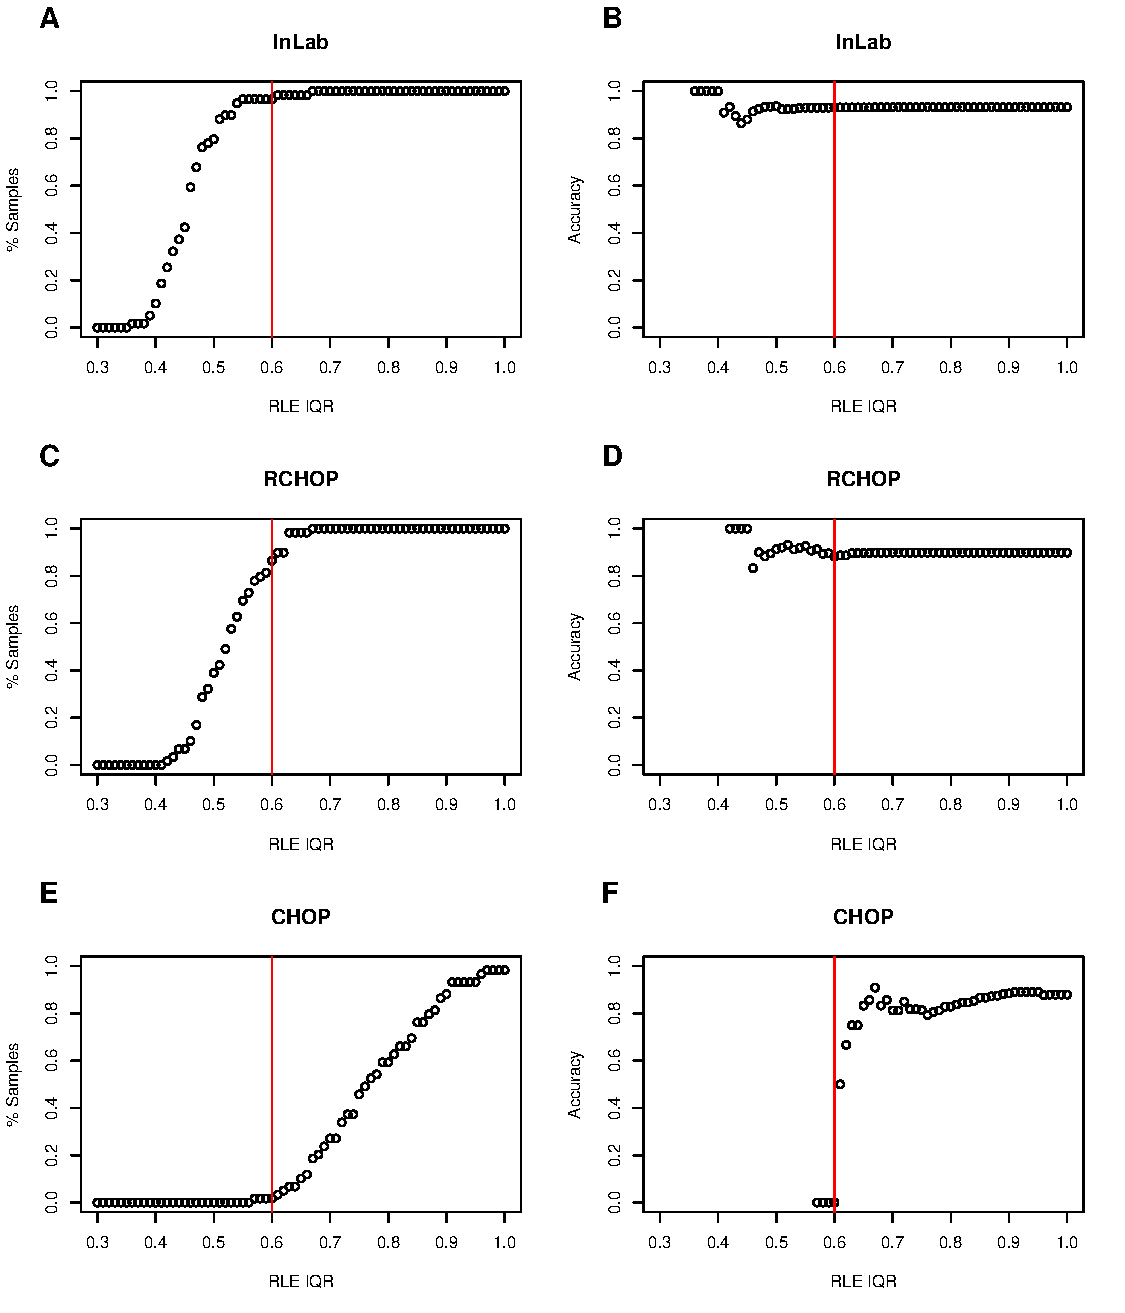
\includegraphics[width=0.8\textwidth]{figures/chep_rle_classification_abcgcb.pdf}
	\end{center}
	\caption{Proportion samples retained and accuracy of ABC/GCB classification (percent similar with cohort based) against increasing RLE IQR thresholds for different references in CHEPRETRO. The vertical line marks the suggested threshold of 0.6}
	\label{fig:chep_rle_clas_abcgcb}
\end{figure}

\begin{figure}
	\begin{center}
		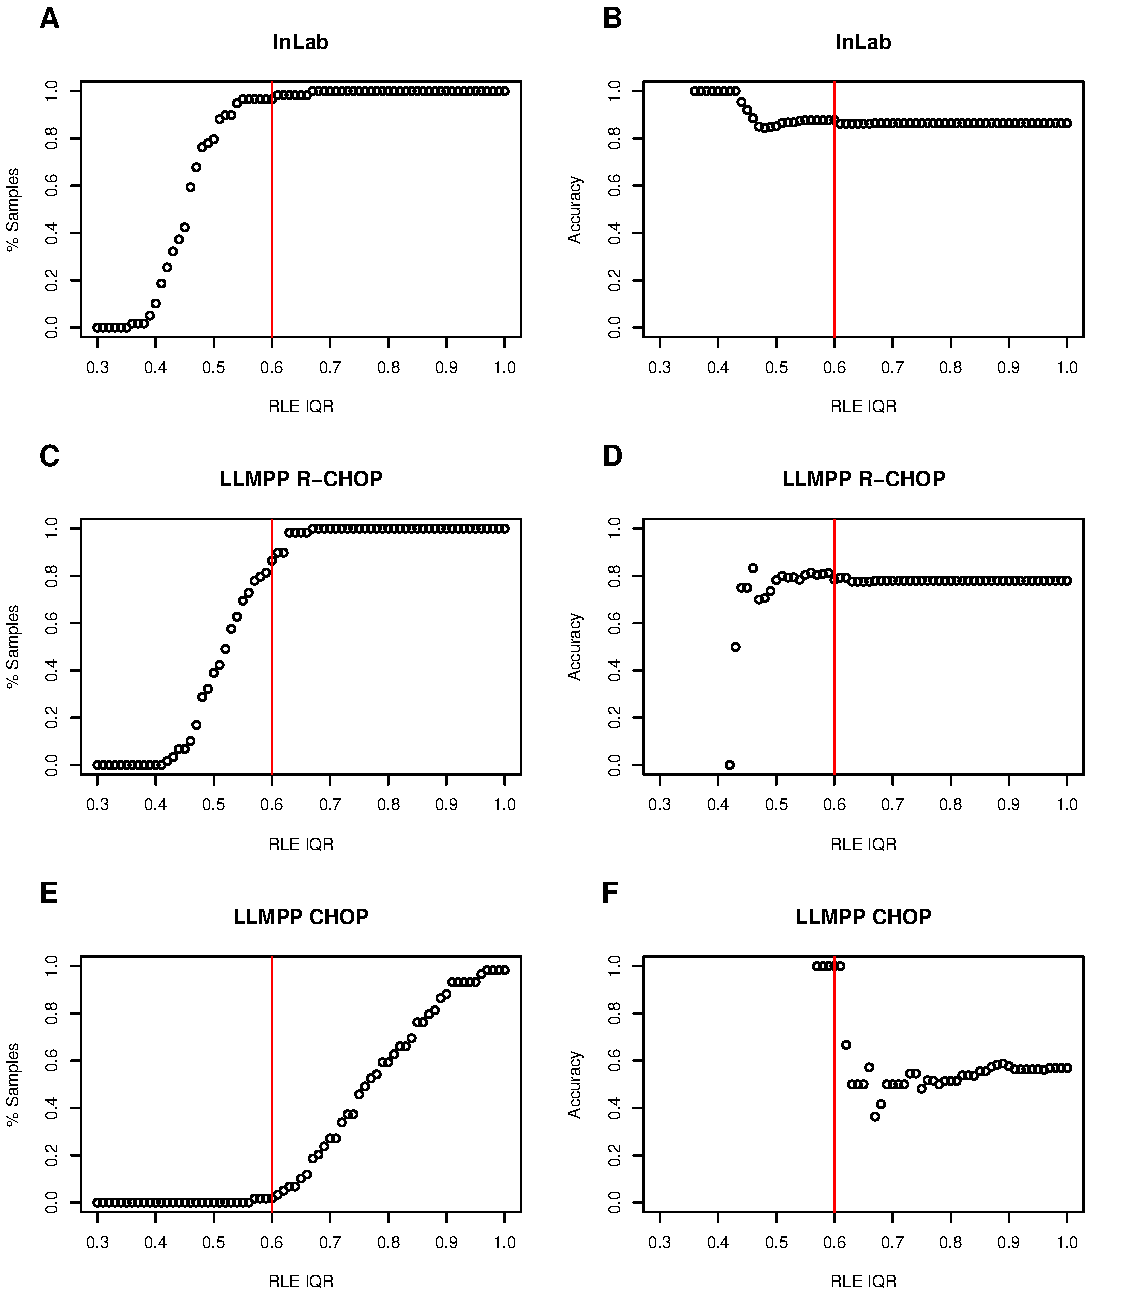
\includegraphics[width=0.8\textwidth]{figures/chep_rle_classification_regs.pdf}
	\end{center}
	\caption{Proportion samples retained and accuracy of REGS(combined) classification (percent similar with cohort based) against increasing RLE IQR thresholds for different references in CHEPRETRO. The vertical line marks the suggested threshold of 0.6}
	\label{fig:chep_rle_clas_regs}
\end{figure}

\begin{figure}
	\begin{center}
		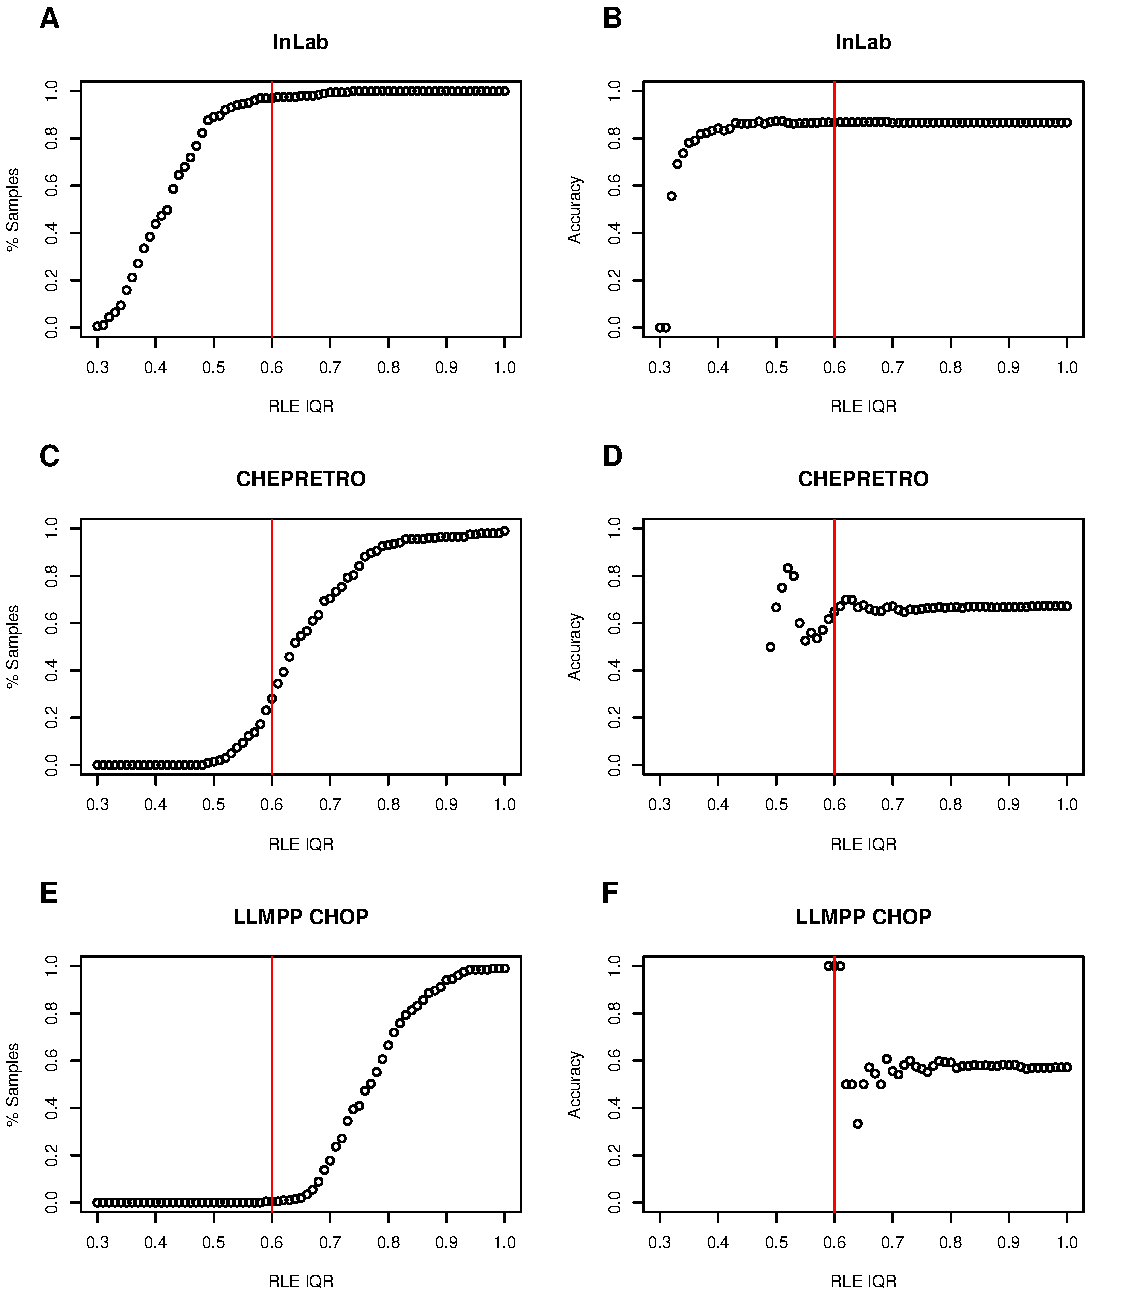
\includegraphics[width=0.8\textwidth]{figures/RCHOP_rle_classification_bags.pdf}
	\end{center}
	\caption{Proportion samples retained and accuracy of BAGS classification (percent similar with cohort based) against increasing RLE IQR thresholds for different references in RCHOP. The vertical line marks the suggested threshold of 0.6}
	\label{fig:RCHOP_rle_clas_bags}
\end{figure}

\begin{figure}
	\begin{center}
		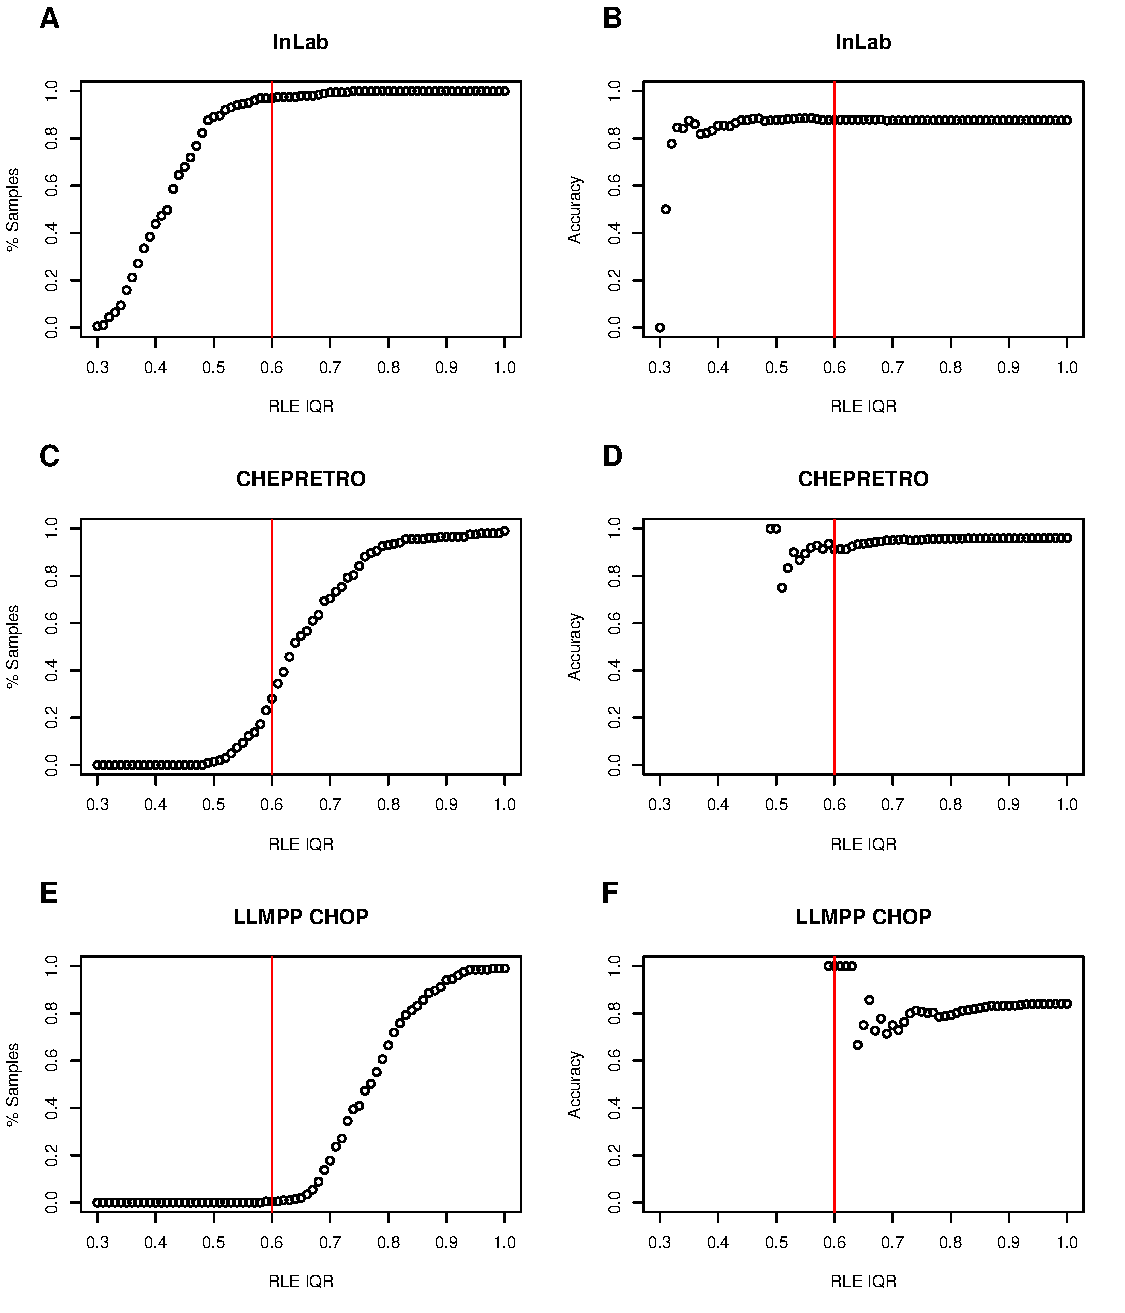
\includegraphics[width=0.8\textwidth]{figures/RCHOP_rle_classification_abcgcb.pdf}
	\end{center}
	\caption{Proportion samples retained and accuracy of ABC/GCB classification (percent similar with cohort based) against increasing RLE IQR thresholds for different references in RCHOP. The vertical line marks the suggested threshold of 0.6}
	\label{fig:RCHOP_rle_clas_abcgcb}
\end{figure}

\begin{figure}
	\begin{center}
		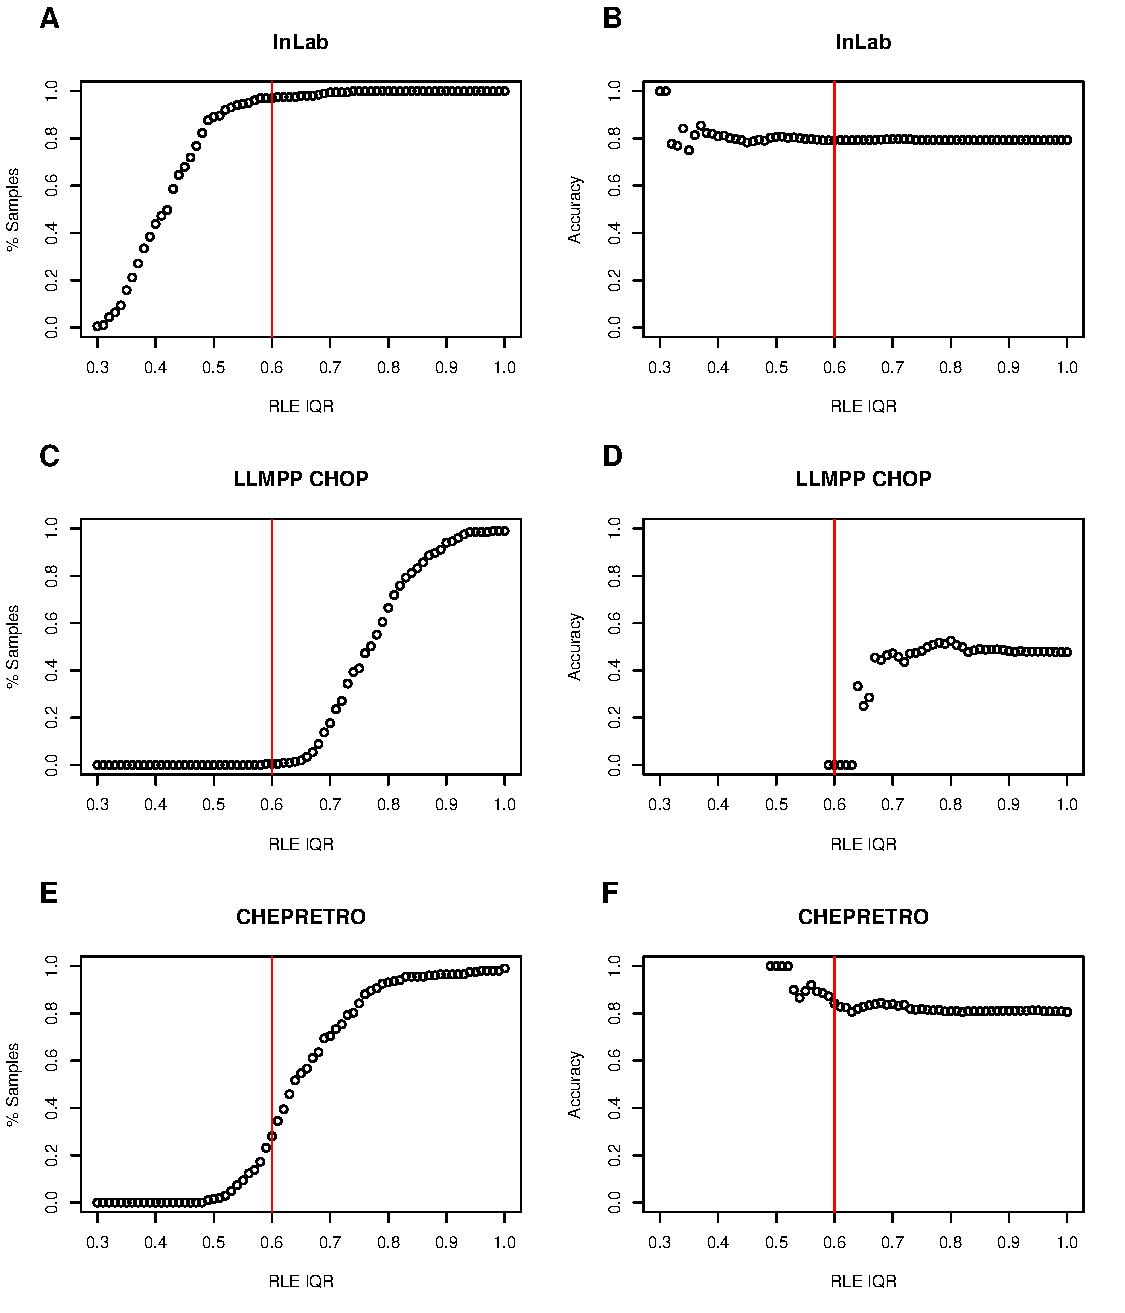
\includegraphics[width=0.8\textwidth]{figures/RCHOP_rle_classification_regs.pdf}
	\end{center}
	\caption{Proportion samples retained and accuracy of REGS(combined) classification (percent similar with cohort based) against increasing RLE IQR thresholds for different references in RCHOP. The vertical line marks the suggested threshold of 0.6}
	\label{fig:RCHOP_rle_clas_regs}
\end{figure}
